

 \maboite{\BS{usepackage}\AC{pgfplots} \cite {pgfplots} }
\label{pgfplots}


\SbSSCT{Courbes 2 D}{2D Graph}

\subsubsection{Axes}

\begin{tabular}{|c|c|c|c|} \hline 

 \multicolumn{4}{|c|}{ \RRP{4-1}}  
 \\ \hline 
\begin{tikzpicture}[scale=.5,blue]
\begin{axis}
...
\end{axis}
\end{tikzpicture}
&
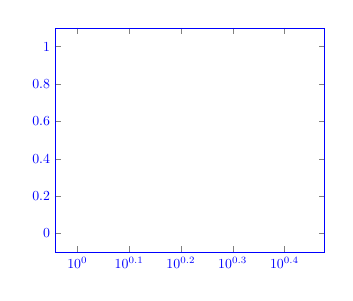
\begin{tikzpicture}[scale=.5,blue]
\begin{semilogxaxis}
...
\end{semilogxaxis}
\end{tikzpicture}
&
\begin{tikzpicture}[scale=.5,blue]
\begin{semilogyaxis}

\end{semilogyaxis}
\end{tikzpicture}
&
\begin{tikzpicture}[scale=.5,blue]
\begin{loglogaxis}

\end{loglogaxis}
\end{tikzpicture}
\\ \hline 
\ESS{axis} & \ESS{semilogxaxis} & \ESS{semilogyaxis} & \ESS{loglogaxis} \\
& & &\\

\BS{end}\AC{axis} & \BS{end}\AC{semilogxaxis} & \BS{end}\AC{semilogyaxis} & \BS{end}\AC{loglogaxis}
\\ \hline 
\end{tabular}


\SbSSCT{Tracé de la courbe}{Drawing of the graph}


\begin{tabular}{|c|c|c|} \hline 
 \multicolumn{3}{|c|}{ \RRP{4-2}}  
 \\ \hline 
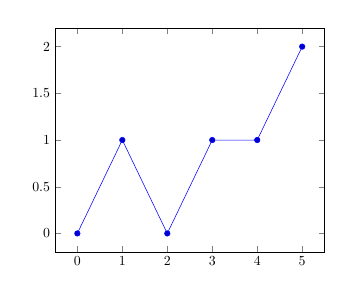
\begin{tikzpicture}[scale=.5]
\begin{axis}
\addplot coordinates {(0,0) (1,1) (2,0) (3,1) (4,1) (5,2)};
\end{axis}
\end{tikzpicture}
&
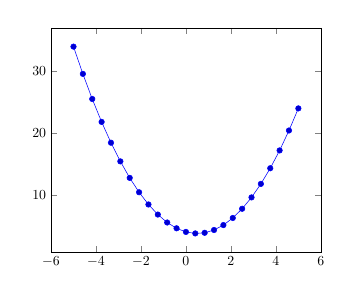
\begin{tikzpicture}[scale=.5]
\begin{axis}
\addplot {x^2 - x +4};
\end{axis}
\end{tikzpicture}
& 

\\ \hline 
\BSS{addplot} coordinates  & \BSS{addplot}  \AC{x\^{}2 - x +4}; & \BSS{addplot}  gnuplot[id=sin]\AC{sin(x)};\\
\AC{(0,0) (1,1) (2,0) (3,1) (4,1) (5,2)}; & &
\\ \hline 
\end{tabular}

\bigskip
\begin{tabular}{|c|c|c|c|} \hline 
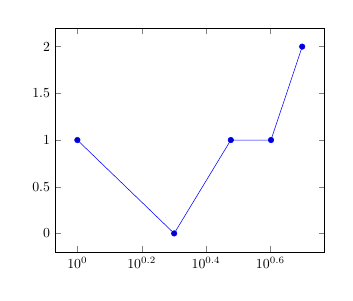
\begin{tikzpicture}[scale=.5]
\begin{semilogxaxis}
\addplot coordinates {(0,0) (1,1) (2,0) (3,1) (4,1) (5,2)};
\end{semilogxaxis}
\end{tikzpicture}
&
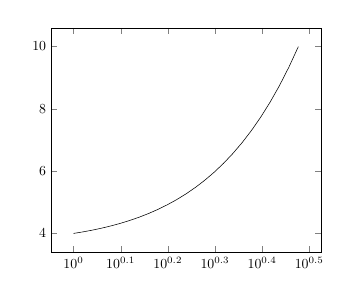
\begin{tikzpicture}[scale=.5]
\begin{semilogxaxis}
\addplot[domain=1:3] {x^2 - x +4};
\end{semilogxaxis}
\end{tikzpicture}
& 
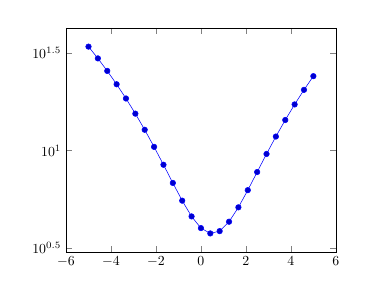
\begin{tikzpicture}[scale=.5]
\begin{semilogyaxis}
\addplot {x^2 - x +4};
\end{semilogyaxis}
\end{tikzpicture}
\\ \hline 
axes : \RDD{semilogxaxis} & axes : \RDD{semilogxaxis} & axes : \RDD{semilogyaxis }
\\ \hline
\BSS{addplot} coordinates  & \BSS{addplot}  \AC{x\^{}2 - x +4}; & \BSS{addplot}  \AC{x\^{}2 - x +4};\\
\AC{(0,0) (1,1) (2,0) (3,1) (4,1) (5,2)}; & &
\\ \hline 
\end{tabular}
\bigskip

%\begin{tabular}{|c|c|c|c|} \hline 
%\begin{tikzpicture}[scale=.5]
%\begin{axis}
%\addplot[red,dashed]  file {table2.dat};
%\addplot[surf]  file {table2.dat};
%\end{axis}
%\end{tikzpicture}
%&
%\begin{tikzpicture}[scale=.5]
%\begin{axis}
%\addplot[red,dashed]  file {table2.dat};
%\addplot[mesh]  file {table2.dat};
%\end{axis}
%\end{tikzpicture}
%&
%\begin{tikzpicture}[scale=.5]
%\begin{axis}
%\addplot[red,dashed]  file {table2.dat};
%\addplot[patch]  file {table2.dat};
%\end{axis}
%\end{tikzpicture}
%\\ \hline 
%patch type=triangle & patch type=rectangle & patch type=line
%\\ \hline 
%\end{tabular}




\begin{tabular}{|c|c|c|c|} \hline 
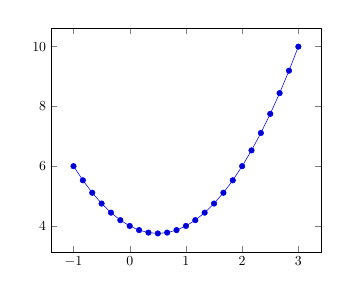
\begin{tikzpicture}[scale=.5]
\begin{axis}[domain=-1:3]
\addplot {x^2 - x +4};
\end{axis}
\end{tikzpicture}
&
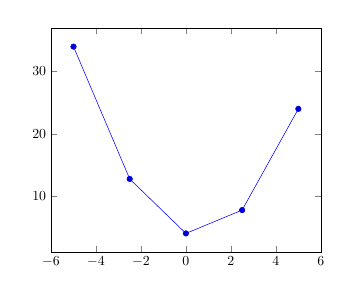
\begin{tikzpicture}[scale=.5]
\begin{axis}[samples=5]
\addplot {x^2 - x +4};
\end{axis}
\end{tikzpicture}
&
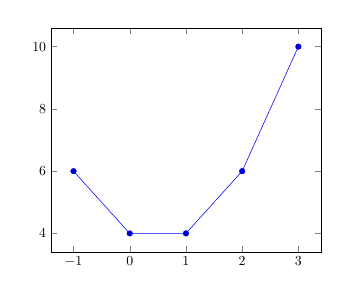
\begin{tikzpicture}[scale=.5]
\begin{axis}[domain=-1:3,samples=5]
\addplot {x^2 - x +4};
\end{axis}
\end{tikzpicture}
\\ \hline 
\BS{begin}\AC{axis}[\RDD{domain}=-1:3] &\BS{begin}\AC{axis}[\RDD{samples}=5] & \BS{begin}\AC{axis}[\RDD{domain}=-1:3,\RDD{samples}=5] 
\\ \hline 
\end{tabular}

\begin{tabular}{|c|c|c|c|} \hline 
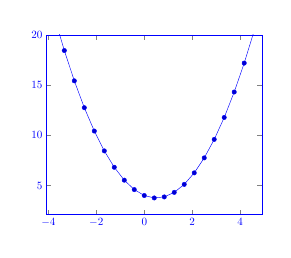
\begin{tikzpicture}[scale=.4]
\begin{axis}[ymax=20,blue]
\addplot {x^2 - x +4};
\end{axis}
\end{tikzpicture}
&
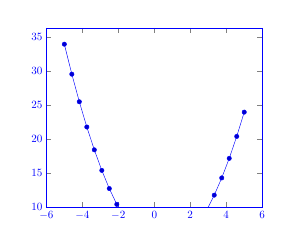
\begin{tikzpicture}[scale=.4]
\begin{axis}[ymin=10,blue]
\addplot {x^2 - x +4};
\end{axis}
\end{tikzpicture}
&

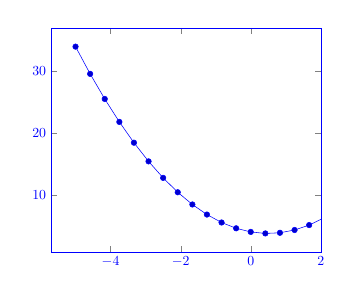
\begin{tikzpicture}[scale=.5]
\begin{axis}[xmax=2,blue]
\addplot {x^2 - x +4};
\end{axis}
\end{tikzpicture}
&
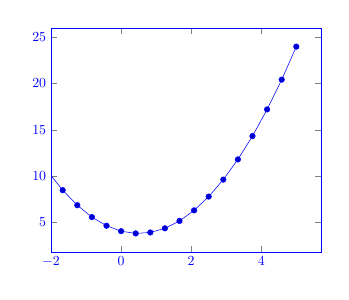
\begin{tikzpicture}[scale=.5]
\begin{axis}[xmin=-2,blue]
\addplot {x^2 - x +4};
\end{axis}
\end{tikzpicture}
\\ \hline 
\RDD{ymax}=20 & \RDD{ymin}=10 & \RDD{xmax}=2 & \RDD{xmin}=-2
\\ \hline
\end{tabular}

\SbSbSSCT{Dimension unitaire en X et Y}{Xunit and Yunit}

\begin{tabular}{|c|c|c|c|} \hline 
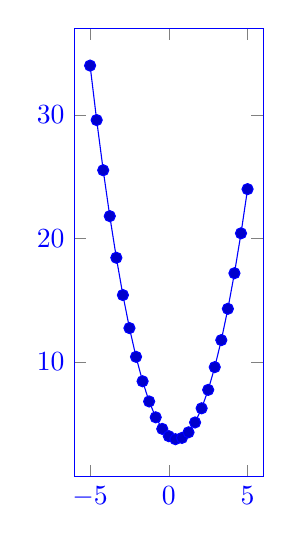
\begin{tikzpicture}
\begin{axis}[x=.2cm,blue]
 \addplot {x^2 - x +4};
\end{axis}
\end{tikzpicture}
&
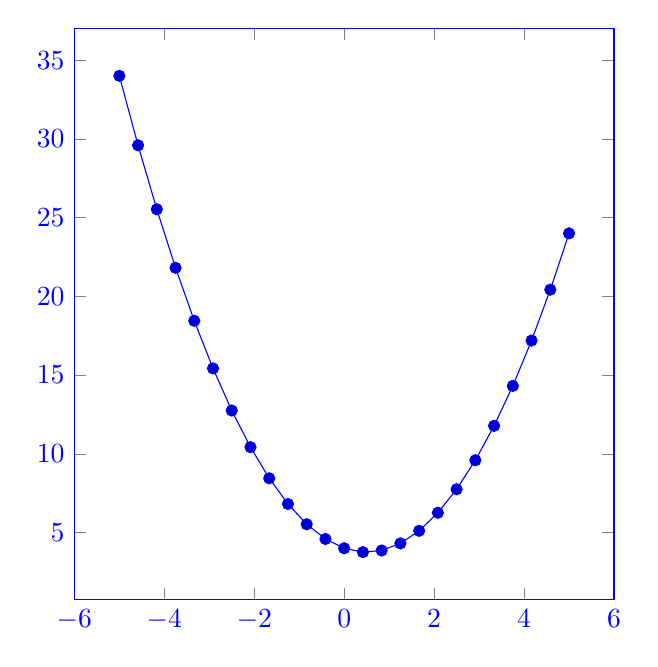
\begin{tikzpicture}
\begin{axis}[y=.2cm,blue]
 \addplot {x^2 - x +4};
\end{axis}
\end{tikzpicture}
&
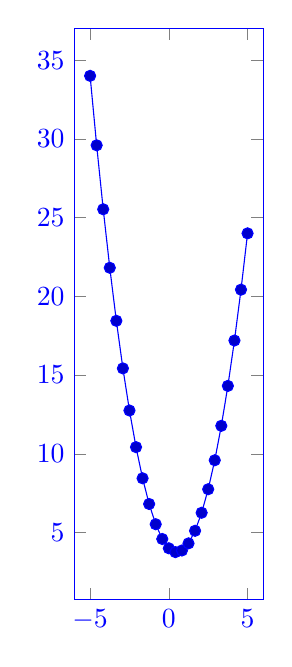
\begin{tikzpicture}
\begin{axis}[x=.2cm,y=.2cm,blue]
 \addplot {x^2 - x +4};
\end{axis}
\end{tikzpicture}

\\ \hline 
\BS{begin}\AC{axis}[\RDD{x}=.2cm] & \BS{begin}\AC{axis}[\RDD{y}=.2cm]& \BS{begin}\AC{axis}[\RDD{x}=.2cm,\RDD{y}=.2cm]
\\ \hline 
\end{tabular}

\SbSbSSCT{Type de graphiques}{Graph type}

\begin{tabular}{|c|c|c|c|} \hline 
\begin{tikzpicture}[scale=.5]
\begin{axis}[const plot,blue]
\addplot file {table2.dat};
\end{axis}
\end{tikzpicture}
&
\begin{tikzpicture}[scale=.5]
\begin{axis}[const plot mark right,blue]
\addplot  file {table2.dat};
\end{axis}
\end{tikzpicture}
&
\begin{tikzpicture}[scale=.5]
\begin{axis}[const plot mark mid,blue]
\addplot  file {table2.dat};
\end{axis}
\end{tikzpicture}
\\ \hline 
\RDD{const plot} & \RDD{const plot mark right} & \RDD{const plot mark mid}
\\ \hline 
\end{tabular}


\begin{tabular}{|c|c|c|c|} \hline 
\begin{tikzpicture}[scale=.5]
\begin{axis}[jump mark left,blue]
\addplot file {table2.dat};
\end{axis}
\end{tikzpicture}
&
\begin{tikzpicture}[scale=.5]
\begin{axis}[jump mark right,blue]
\addplot  file {table2.dat};
\end{axis}
\end{tikzpicture}
&
\begin{tikzpicture}[scale=.5]
\begin{axis}[jump mark mid,blue]
\addplot  file {table2.dat};
\end{axis}
\end{tikzpicture}
\\ \hline 
\RDD{jump mark left} & \RDD{jump mark right} & \RDD{jump mark mid}
\\ \hline 
\end{tabular}

\begin{tabular}{|c|c|c|c|} \hline 
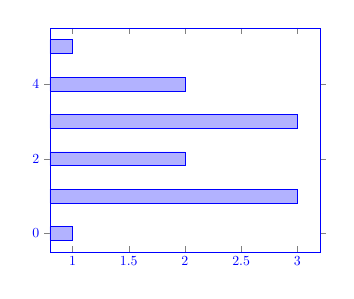
\begin{tikzpicture}[scale=.5]
\begin{axis}[xbar,blue]
\addplot coordinates {(1,0) (3,1) (2,2) (3,3) (2,4) (1,5)};
\end{axis}
\end{tikzpicture}
&
\begin{tikzpicture}[scale=.5]
\begin{axis}[ybar,blue]
\addplot  file {table2.dat};
\end{axis}
\end{tikzpicture}
&
\begin{tikzpicture}[scale=.5]
\begin{axis}[ybar interval,blue]
\addplot  file {table2.dat};
\end{axis}
\end{tikzpicture}
\\ \hline 
\RDD{xbar} & \RDD{ybar} & \RDD{ybar interval}
\\ \hline 
\end{tabular}


\begin{tabular}{|c|c|c|c|} \hline 
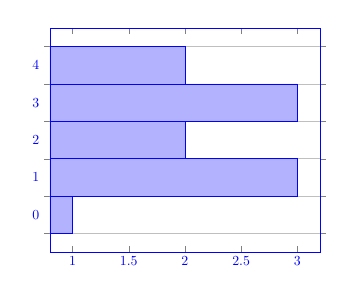
\begin{tikzpicture}[scale=.5]
\begin{axis}[xbar interval,blue]
\addplot  coordinates {(1,0) (3,1) (2,2) (3,3) (2,4) (1,5)};
\end{axis}
\end{tikzpicture}
&
\begin{tikzpicture}[scale=.5]
\begin{axis}[xcomb,blue]
\addplot  file {table2.dat};
\end{axis}
\end{tikzpicture}
&
\begin{tikzpicture}[scale=.5]
\begin{axis}[ycomb,blue]
\addplot  file {table2.dat};
\end{axis}
\end{tikzpicture}
\\ \hline 
\RDD{xbar interval} & \RDD{xcomb} & \RDD{ycomb}
\\ \hline 
\end{tabular}


\begin{tabular}{|c|c|c|c|} \hline 
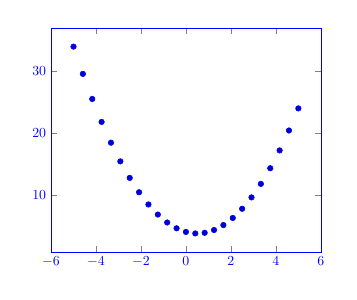
\begin{tikzpicture}[scale=.5]
\begin{axis}[only marks,blue]
\addplot {x^2 - x +4};
\end{axis}
\end{tikzpicture}
&
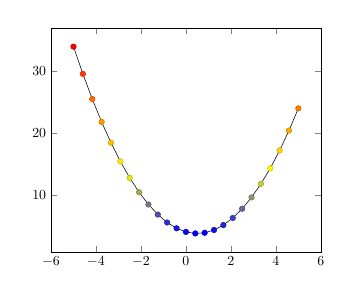
\begin{tikzpicture}[scale=.5]
\begin{axis}
\addplot [scatter] {x^2 - x +4};
\end{axis}
\end{tikzpicture}
&

\\ \hline 
\RDD{only marks} & \RDD{scatter} & \RDD{mesh}
\\ \hline
\end{tabular}


\smallskip
\begin{tabular}{|c|c|c|c|} \hline 
\multicolumn{2}{|c|}{  \BS{addplot}  [\RDD{quiver}=\AC{u=1,v=2*x}],->,samples=5,blue,ultra thick]  \AC{x\^{}2 - x +4};   }
\\ \hline
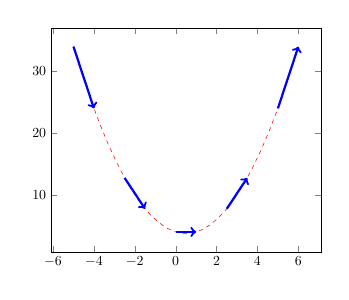
\begin{tikzpicture}[scale=.5]

\begin{axis}
\addplot [red,dashed,no marks] {x^2 - x +4};
\addplot [quiver={u=1,v=2*x},->,samples=5,blue,ultra thick] {x^2 - x +4};
\end{axis}
\end{tikzpicture}
&
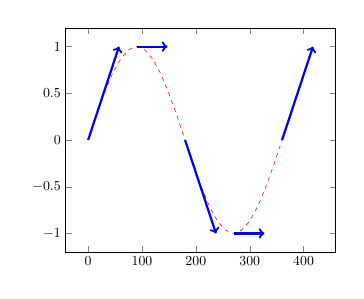
\begin{tikzpicture}[scale=.5,domain=0:360,ultra thick]
\begin{axis}
\addplot [red,dashed,no marks] (\x,{sin(\x)});
\addplot [quiver={u=180/3.14,v=cos(x)},->,samples=5,blue,ultra thick] (\x,{sin(\x)});
\end{axis}
\end{tikzpicture}
\\ \hline
\RDD{quiver}={u=1,v=2*x} & \RDD{quiver}=\AC{u=180/3.14,v=cos(x)}
\\ \hline
\multicolumn{2}{|c|}{ \dft :   u=0  et  v = 0}
\\ \hline
\end{tabular}




%\subsection{stack}
\smallskip
\begin{tabular}{|c|c|c|c|} \hline 
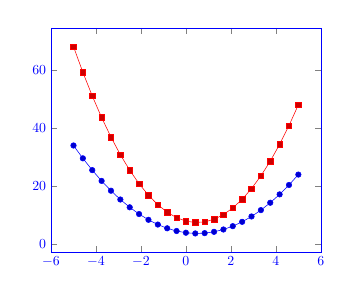
\begin{tikzpicture}[scale=.5]
\begin{axis}[stack plots=y,blue]
\addplot {x^2 - x +4};
\addplot {x^2 - x +4};
\end{axis}
\end{tikzpicture}
&

\begin{tikzpicture}[scale=.5]
\begin{axis}[stack plots=y,blue]
\addplot  file {table2.dat};
\addplot   file {table2.dat};
\end{axis}
\end{tikzpicture}
&

\begin{tikzpicture}[scale=.5]
\begin{axis}[ybar stacked,blue]
\addplot  file {table2.dat};
\addplot   file {table2.dat};
\end{axis}
\end{tikzpicture}
\\ \hline
[\RDD{stack plots}=y,blue] & [\RDD{stack plots=y},blue] & [\RDD{ybar stacked},blue]
\\ \hline
\end{tabular}

\bigskip
\begin{tabular}{|c|c|c|c|} \hline 
\begin{tikzpicture}[scale=.5]
\begin{axis}[stack plots=y,area style]
\addplot  file {table2.dat};
\addplot   file {table2.dat};
\end{axis}
\end{tikzpicture}
&
\begin{tikzpicture}[scale=.5]
\begin{axis}[const plot,stack plots=y,area style]
\addplot  file {table2.dat};
\addplot   file {table2.dat};
\end{axis}
\end{tikzpicture}
&
\begin{tikzpicture}[scale=.5]
\begin{axis}[stack plots=y,area style,smooth]
\addplot  file {table2.dat};
\addplot   file {table2.dat};
\end{axis}
\end{tikzpicture}
\\ \hline
[stack plots=y,area style] & [const plot,stack plots=y,area style] & [stack plots=y,area style,smooth]
\\ \hline

\end{tabular}


\bigskip

\begin{tabular}{|c|c|c|c|} \hline 
\multicolumn{3}{|c|}{  \BS{addplot}  [\RDD{error bars/y dir}=both,\RDD{error bars/y fixed} =2.5]  \AC{x\^{}2 - x +4};   }
\\ \hline

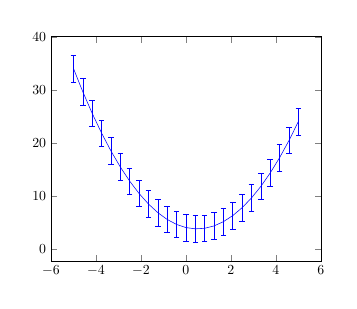
\begin{tikzpicture}[scale=.5]
\begin{axis}
\addplot [error bars/y dir =both,error bars/y fixed =2.5,blue]{x^2 - x +4};
\end{axis}
\end{tikzpicture}
&
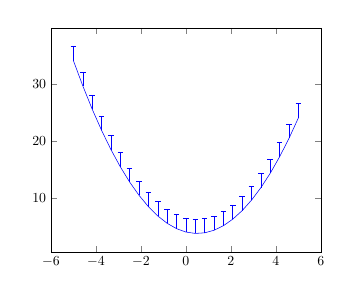
\begin{tikzpicture}[scale=.5]
\begin{axis}
\addplot [error bars/y dir =plus,error bars/y fixed =2.5,blue]{x^2 - x +4};
\end{axis}
\end{tikzpicture}
&
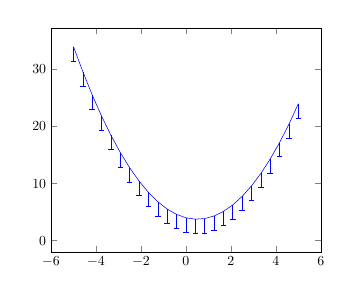
\begin{tikzpicture}[scale=.5]
\begin{axis}
\addplot [error bars/y dir =minus,error bars/y fixed =2.5,blue]{x^2 - x +4};
\end{axis}
\end{tikzpicture}
\\ \hline
\RDD{error bars/y dir} =both & \RDD{error bars/y dir} =plus & \RDD{error bars/y dir} =minus
\\ \hline
\end{tabular}





\bigskip

\begin{tabular}{|c|c|c|c|} \hline 
\multicolumn{3}{|c|}{  \BS{addplot}  [\RDD{error bars/x dir}=both,\RDD{error bars/x fixed} =.5]  \AC{x\^{}2 - x +4};   }
\\ \hline
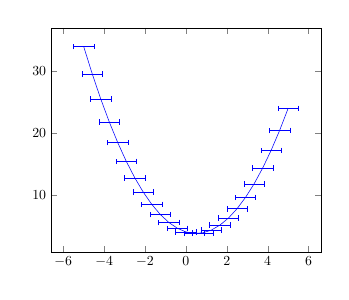
\begin{tikzpicture}[scale=.5]
\begin{axis}
\addplot [error bars/x dir =both,error bars/x fixed =.5,blue]{x^2 - x +4};
\end{axis}
\end{tikzpicture}
&
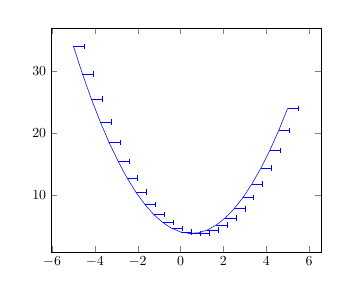
\begin{tikzpicture}[scale=.5]
\begin{axis}
\addplot [error bars/x dir =plus,error bars/x fixed =.5,blue]{x^2 - x +4};
\end{axis}
\end{tikzpicture}
&
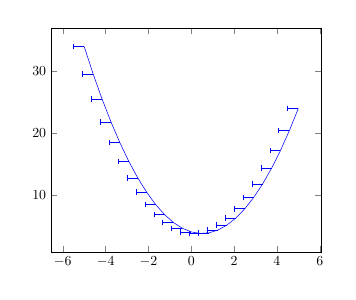
\begin{tikzpicture}[scale=.5]
\begin{axis}
\addplot [error bars/x dir =minus,error bars/x fixed =.5,blue]{x^2 - x +4};
\end{axis}
\end{tikzpicture}
\\ \hline
\RDD{error bars/x dir} =both &\RDD{ error bars/x dir} =plus & \RDD{error bars/x dir} =minus
\\ \hline
\end{tabular}

\bigskip
\begin{tabular}{|c|c|c|c|} \hline 
\multicolumn{3}{|c|}{  \BS{addplot}  [\RDD{error bars/y dir}=both,\RDD{error bars/x fixed relative} =.2]  \AC{x\^{}2 - x +4};   }
\\ \hline

\begin{tikzpicture}[scale=.5]

\begin{axis}
\addplot [error bars/y dir =both,error bars/y fixed relative =.2,blue]{x^2 - x +4};
\end{axis}
\end{tikzpicture}
&
\begin{tikzpicture}[scale=.5]
\begin{axis}
\addplot [error bars/y dir =plus,error bars/y fixed relative =1,blue]{x^2 - x +4};
\end{axis}
\end{tikzpicture}
&
\begin{tikzpicture}[scale=.5]
\begin{axis}
\addplot [error bars/x dir =minus,error bars/x fixed relative =.2,blue]{x^2 - x +4};
\end{axis}
\end{tikzpicture}
\\ \hline
\RDD{error bars/y fixed relative} =.2 & \RDD{error bars/y fixed relative} =1 & \RDD{error bars/x fixed relative} =.2
\\ \hline
\end{tabular}


\SbSSCT{Habillage du graphe}{Graph information}

\SbSbSSCT{Titres}{Titles}

\begin{tabular}{|c|c|c|c|} \hline 
\begin{tikzpicture}[scale=.5]
\begin{axis}[xlabel=axe X,blue]
...
\end{axis}
\end{tikzpicture}
&
\begin{tikzpicture}[scale=.5]
\begin{axis}[ylabel=axe Y,blue]
...
\end{axis}
\end{tikzpicture}
&
\begin{tikzpicture}[scale=.5]
\begin{axis}[title=Titre du graphe,blue]
 
\end{axis}
\end{tikzpicture}


\\ \hline 
\BS{begin}\AC{axis}[\RDD{xlabel}=axe X] & \BS{begin}\AC{axis}[\RDD{ylabel}=axe Y] & \BS{begin}\AC{axis}[\RDD{title}=Titre du graphe]
\\ \hline 
\end{tabular}

\SbSbSSCT{Légende}{Legend}

\begin{tabular}{|c|c|c|c|} \hline 
\begin{tikzpicture}[blue ,baseline=0pt,scale=.5]
\begin{axis}
\addplot {x^2 - x +4};
\addplot {x^2 - x +2};
\addplot {x^2 - x };
\addplot {x^2 - x -2 };
\addplot {x^2 - x -4 };
\legend{$x^2 - x +4$,$x^2 - x +2$,$x^2 - x $,$x^2 - x -2 $,$x^2 - x -4 $}
\end{axis}
\end{tikzpicture}
&
\parbox[c]{10cm}{
\BS{begin}\AC{axis}\\
\BSS{addplot} \AC{x\^{}2 - x +4};\\
\BSS{addplot} \AC{x\^{}2 - x +2};\\
\BSS{addplot} \AC{x\^{}2 - x };\\
\BSS{addplot} \AC{x\^{}2 - x -2 };\\
\BSS{addplot} \AC{x\^{}2 - x -4 };\\

\BSS{legend}\AC{\$x\^{}2 - x +4\$,\$x\^{}2 - x +2\$,\$x\^{}2 - x \$,\$x\^{}2 - x -2 \$,\$x\^{}2 - x -4 \$}\\
\BS{end}\AC{axis}}
\\ \hline 
 
\begin{tikzpicture}[blue ,baseline=0pt,scale=.5]
\begin{axis}[legend entries={$x^2 - x +4$,$x^2 - x +2$,$x^2 - x $,$x^2 - x -2 $,$x^2 - x -4 $}]
\addplot {x^2 - x +4};
\addplot {x^2 - x +2};
\addplot {x^2 - x };
\addplot {x^2 - x -2 };
\addplot {x^2 - x -4 };

\end{axis}
\end{tikzpicture}
&
\parbox[c]{10cm}{
\BS{begin}\AC{axis}[\RDD{legend entries}= \AC{\$ x\^{}2 - x +4 \$,\$ x\^{}2 - x +2 \$,\$ x\^{}2 - x \$,\$ x\^{}2 - x -2 \$,\$ x\^{}2 - x -4 \$} ] \\

\BSS{addplot} \AC{x\^{}2 - x +4};\\
\BSS{addplot} \AC{x\^{}2 - x +2};\\
\BSS{addplot} \AC{x\^{}2 - x };\\
\BSS{addplot} \AC{x\^{}2 - x -2 };\\
\BSS{addplot} \AC{x\^{}2 - x -4 };\\
\BS{end}\AC{axis}}
\\ \hline 
\end{tabular}


Options

\begin{tabular}{|c|c|c|c|} \hline 
\begin{tikzpicture}[blue ,baseline=0pt,scale=.5]
\begin{axis}[legend entries={$x^2 - x +4$,$x^2 - x +2$,$x^2 - x $,$x^2 - x -2 $,$x^2 - x -4 $},legend style={font=\tiny}]
\addplot {x^2 - x +4};
\addplot {x^2 - x +2};
\addplot {x^2 - x };
\addplot {x^2 - x -2 };
\addplot {x^2 - x -4 };
\end{axis}
\end{tikzpicture}
&
\begin{tikzpicture}[blue ,baseline=0pt,scale=.5]
\begin{axis}[legend entries={$x^2 - x +4$,$x^2 - x +2$,$x^2 - x $,$x^2 - x -2 $,$x^2 - x -4 $},legend style={draw=none}]
\addplot {x^2 - x +4};
\addplot {x^2 - x +2};
\addplot {x^2 - x };
\addplot {x^2 - x -2 };
\addplot {x^2 - x -4 };
\end{axis}
\end{tikzpicture}
&
\begin{tikzpicture}[blue ,baseline=0pt,scale=.5]
\begin{axis}[legend entries={$x^2 - x +4$,$x^2 - x +2$},legend style={shape=ellipse}]
\addplot {x^2 - x +4};
\addplot {x^2 - x +2};
\end{axis}
\end{tikzpicture}
\\ \hline 
\RDD{legend style}=\AC{\RDD{font}=\BS{tiny}} & \RDD{legend style}=\AC{\RDD{draw}=none} & \RDD{legend style}=\AC{\RDD{shape}=ellipse} 
\\ \hline 
\end{tabular}




\bigskip
\begin{tabular}{|c|c|c|c|} \hline 
\begin{tikzpicture}[blue ,baseline=0pt,scale=.5]
\begin{axis}[legend style={at={(.5,.5)}}]
\addplot {x^2 - x +4};
\addplot {x^2 - x +2};
\addplot {x^2 - x };
\addplot {x^2 - x -2 };
\addplot {x^2 - x -4 };
\legend{$x^2 - x +4$,$x^2 - x +2$,$x^2 - x $,$x^2 - x -2 $,$x^2 - x -4 $}
\end{axis}
\end{tikzpicture}
&
\begin{tikzpicture}[blue ,baseline=0pt,scale=.5]
\begin{axis}[legend style={legend pos=outer north east}]
\addplot {x^2 - x +4};
\addplot {x^2 - x +2};
\addplot {x^2 - x };
\addplot {x^2 - x -2 };
\addplot {x^2 - x -4 };
\legend{$x^2 - x +4$,$x^2 - x +2$,$x^2 - x $,$x^2 - x -2 $,$x^2 - x -4 $}
\end{axis}
\end{tikzpicture}
\\ \hline 
legend style=\AC{\RDD{at}=\AC{(.5,.5)}} & legend style=\AC{\RDD{legend pos}=outer north east}
\\ \hline 
\end{tabular}

\bigskip
\begin{tabular}{|c|c|c|c|} \hline 
\begin{tikzpicture}[blue ,baseline=0pt,scale=.5]
\begin{axis}[legend style={legend columns=2}]
\addplot {x^2 - x +4};
\addplot {x^2 - x +2};
\addplot {x^2 - x };
\addplot {x^2 - x -2 };
\addplot {x^2 - x -4 };
\legend{A,B,C,D,E}
\end{axis}
\end{tikzpicture}
&
\begin{tikzpicture}[blue ,baseline=0pt,scale=.5]
\begin{axis}[legend style={legend columns=3}]
\addplot {x^2 - x +4};
\addplot {x^2 - x +2};
\addplot {x^2 - x };
\addplot {x^2 - x -2 };
\addplot {x^2 - x -4 };
\legend{A,B,C,D,E}
\end{axis}
\end{tikzpicture}
&
\begin{tikzpicture}[blue ,baseline=0pt,scale=.5]
\begin{axis}[legend style={legend columns=-1}]
\addplot {x^2 - x +4};
\addplot {x^2 - x +2};
\addplot {x^2 - x };
\addplot {x^2 - x -2 };
\addplot {x^2 - x -4 };
\legend{A,B,C,D,E}
\end{axis}
\end{tikzpicture}

\\ \hline 
legend style=\AC{\RDD{legend columns}=2} & legend style=\AC{\RDD{legend columns}=3}  & legend style=\AC{\RDD{legend columns}=-1}
\\ \hline 
\end{tabular}

\bigskip

\begin{tabular}{|c|c|c|c|} \hline 
\begin{tikzpicture}[blue ,baseline=0pt,scale=.5]
\begin{axis}[legend cell align=left]
\addplot {x^2 - x +4};
\addplot {x^2 - x +2};
\addplot {x^2 - x };
\addplot {x^2 - x -2 };
\addplot {x^2 - x -4 };
\legend{$x^2 - x +4$,f(x),$x^2 - x $,courbe,Y}
\end{axis}
\end{tikzpicture}
&
\begin{tikzpicture}[blue ,baseline=0pt,scale=.5]
\begin{axis}[legend cell align=center,]
\addplot {x^2 - x +4};
\addplot {x^2 - x +2};
\addplot {x^2 - x };
\addplot {x^2 - x -2 };
\addplot {x^2 - x -4 };
\legend{$x^2 - x +4$,f(x),$x^2 - x $,courbe,Y}
\end{axis}
\end{tikzpicture}
&
\begin{tikzpicture}[blue ,baseline=0pt,scale=.5]
\begin{axis}[legend cell align=right]
\addplot {x^2 - x +4};
\addplot {x^2 - x +2};
\addplot {x^2 - x };
\addplot {x^2 - x -2 };
\addplot {x^2 - x -4 };
\legend{$x^2 - x +4$,f(x),$x^2 - x $,courbe,Y}
\end{axis}
\end{tikzpicture}
\\ \hline 
[\RDD{legend cell align}=left] & [\RDD{legend cell align}=center] & [\RDD{legend cell align}=right]
\\ \hline 
\end{tabular}

\SbSbSSCT{Taille du graphe}{Size of the graph}

\begin{tabular}{|c|c|c|c|} \hline 
\begin{tikzpicture}
\begin{axis}[width=3cm,grid=major,blue]
 \addplot {x^2 - x +4};
\end{axis}
\end{tikzpicture}
&
\begin{tikzpicture}
\begin{axis}[height=5cm,grid=major,blue]
 \addplot {x^2 - x +4};
\end{axis}
\end{tikzpicture}
&
\begin{tikzpicture}
\begin{axis}[width=3cm,height=5cm,grid=major,blue]
 \addplot {x^2 - x +4};
\end{axis}
\end{tikzpicture}

\\ \hline
\RDD{width}=3cm & \RDD{height}=5cm & \RDD{width}=3cm,\RDD{height}=5cm
\\ \hline 


\end{tabular}

\SbSbSSCT{Quadrillage}{Grids}

\begin{tabular}{|c|c|c|c|} \hline 
\begin{tikzpicture}[scale=.5]
\begin{axis}[xmajorgrids=true,blue]
\addplot {x^2 - x +4};
\end{axis}
\end{tikzpicture}
&
\begin{tikzpicture}[scale=.5]
\begin{axis}[ymajorgrids=true,blue]
\addplot {x^2 - x +4};
\end{axis}
\end{tikzpicture}
&
\begin{tikzpicture}[scale=.5]
\begin{axis}[grid=major,blue]
\addplot {x^2 - x +4};
\end{axis}
\end{tikzpicture}
\\ \hline 
\BS{begin}\AC{axis}[\RDD{xmajorgrids}=true] &\BS{begin}\AC{axis}[\RDD{ymajorgrids}=true] & \BS{begin}\AC{axis}[\RDD{grid}=major] 
\\ \hline 
\end{tabular}

%\subsubsection{minorgrids}
%
%\begin{tabular}{|c|c|c|c|} \hline 
%\begin{tikzpicture}[scale=.4]
%\begin{loglogaxis}[grid=major,blue]
%\addplot {x^2 - x +4};
%\end{loglogaxis}
%\end{tikzpicture}
%&
%\begin{tikzpicture}[scale=.4]
%\begin{loglogaxis}[grid=both,blue]
%\addplot {x^2 - x +4};
%\end{loglogaxis}
%\end{tikzpicture}
%\\ \hline 
%\end{tabular}

\begin{tabular}{|l|l|c|c|} \hline 
\begin{tikzpicture}
\begin{axis}[nodes near coords,blue,samples=10]
\addplot {x^2 - x +4};
\end{axis}
\end{tikzpicture}
 &
 \begin{tikzpicture}
 \begin{axis}[nodes near coords,blue]
 \addplot file {table2.dat};
 \end{axis}
 \end{tikzpicture}
 \\ \hline 
 \BS{begin}AC{axis}[\RDD{nodes near coords},samples=10] &  \BS{begin}AC{axis}[\RDD{nodes near coords}]\\
 \BS{addplot} \AC{x\^{} 2- x +4}; &   \BS{addplot}  file {table2.dat}; 
 
 \\ \hline  
 \end{tabular}
 

\newpage

